\documentclass[conference]{IEEEtran}

\usepackage{cite}
\usepackage{amsmath,amssymb}
\usepackage{graphicx}
\usepackage{booktabs}
\usepackage{url}
\usepackage{tikz}
\usetikzlibrary{positioning,arrows.meta}
\usepackage{algorithm}
\usepackage{algpseudocode}
\usepackage[hidelinks]{hyperref}

\newcommand{\ASR}{\mathrm{ASR}}
\newcommand{\ACC}{\mathrm{ACC}}
\newcommand{\Texc}{\mathrm{T}}

\setlength{\textfloatsep}{10pt plus 2pt minus 2pt}
\setlength{\floatsep}{8pt plus 2pt minus 2pt}
\setlength{\intextsep}{8pt plus 2pt minus 2pt}
\begin{document}
\bstctlcite{IEEEexample:BSTcontrol}

\title{Revisiting ADFL: An Adversarial Evaluation of GAN-Based Distillation Defenses for Federated Backdoors}

\author{\IEEEauthorblockN{Andrés Uriza Lazo}
\IEEEauthorblockA{urizandres@estudiantec.cr}}

\maketitle

\begin{abstract}
Federated learning (FL) is vulnerable to backdoor attacks, in which a few malicious clients implant a trigger-activated behavior into the global model. Zhu et al.\ proposed ADFL, a server-side defense that seeds a GAN discriminator from the backdoored model, labels generated samples with a small clean teacher, and purifies the model by distillation, reporting a 95\% lower attack success rate (ASR) at accuracy above 90\% \cite{zhu2023adfl}. As no reference implementation exists, I re-implemented ADFL and evaluated it at paper scale (three seeds; MNIST, Fashion-MNIST, CIFAR-10; IID and Dirichlet Non-IID). The MNIST pixel-trigger control reproduces: ASR falls from 1.000 to $0.002\pm0.002$. On Fashion-MNIST Non-IID, a random pixel trigger survives at $0.434\pm0.175$ ASR, with strong seed dependence. On CIFAR-10, GAN-based distillation collapses clean accuracy (0.65 to 0.22--0.23), whereas distillation on real relabeled images removes the backdoor at about 0.72 accuracy, isolating synthetic-data quality as the cause. A bounded adaptive attack shows no measurable advantage over a blind trigger (post-ADFL ASR $0.416\pm0.292$ and $0.373\pm0.353$ versus $0.526\pm0.268$). Accuracy costs of $-0.04$ (MNIST), $-0.16$ (Fashion IID) and $-0.24$ (Fashion Non-IID) stand against the original ``above 90\%'' claim.
\end{abstract}

\begin{IEEEkeywords}
federated learning, backdoor attacks, backdoor defense, generative adversarial networks, knowledge distillation, reproducibility
\end{IEEEkeywords}

%=====================================================================
\section{Introduction}
Federated learning lets many clients train jointly without sharing raw data \cite{mcmahan2017fedavg,kairouz2021advances}, which also keeps the server from inspecting client data or local training. The global model is therefore a target for backdoors: malicious clients train on trigger-stamped samples relabeled to an attacker-chosen class and, in the model-replacement strategy, scale their updates so the aggregate adopts the backdoor \cite{bagdasaryan2020backdoor,bhagoji2019adversarial,sun2019backdoor}. The model then behaves normally on clean inputs but predicts the target class when the trigger is present \cite{gu2017badnets}.

Zhu et al.\ propose ADFL \cite{zhu2023adfl}, a server-side, GAN-based defense \cite{goodfellow2014gan}. The authors report that it lowers ASR by 95\% and keeps accuracy above 90\% on MNIST, Fashion-MNIST, EMNIST, CIFAR-10 and CelebA, outperforming FoolsGold, CONTRA and BaFFLe \cite{fung2020foolsgold,awan2021contra,andreina2021baffle}, including under Non-IID partitions. To my knowledge no code accompanies these claims. I therefore build an independent implementation as a testbed and ask: \emph{where does ADFL break when its assumptions are stressed, what does it cost in clean accuracy, and can a trigger chosen against the defense do better than a generic one?}

The contributions of this paper are the findings of that adversarial evaluation. The ADFL pipeline itself -- the GAN, the clean teacher and the distillation objective -- is Zhu et al.'s; my re-implementation is only the instrument used to obtain the results and is not claimed as a contribution.
\begin{itemize}
\item \textbf{A failure map of ADFL.} A paper-scale evaluation (three seeds; MNIST \cite{lecun1998mnist}, Fashion-MNIST \cite{xiao2017fashion}, CIFAR-10 \cite{krizhevsky2009cifar}; IID and Dirichlet Non-IID partitions \cite{hsu2019noniid}) that locates where the defense holds and where it does not: it holds on MNIST, leaves residual backdoors on Fashion-MNIST (a random $14{\times}14$ patch survives at $0.434\pm0.175$ ASR under Non-IID), and collapses to $0.15$--$0.23$ accuracy on CIFAR-10. The accuracy tax is $-0.04$ to $-0.24$ on grayscale datasets, against the reported ``above 90\%''.
\item \textbf{A trigger-level evasion screen and a trigger-agnostic metric.} The \emph{excess} of post-defense ASR over the clean teacher's own target rate (Eq.~\ref{eq:excess}), which separates a surviving backdoor from a trigger that merely pushes clean inputs to the target, and a screen over 16--19 candidates per dataset (Alg.~\ref{alg:screen}) confirmed by full FL. Conventional pixel and watermark triggers understate what survives; a centralized proxy overstates it (excess $0.944$ versus $0.390$).
\item \textbf{A diagnosis of the failure mechanisms.} A real-data upper-bound gate attributes the CIFAR-10 collapse to synthetic-data quality rather than to distillation; a teacher/GAN partition ablation localizes the Non-IID degradation to the server teacher; an MNIST Non-IID control indicates that partitioning alone is not the cause; and the distillation loss is uninformative about residual backdoor strength. A multi-seed follow-up redraws the partition and teacher per seed.
\item \textbf{A bounded adaptive attack, reported as the negative result it is} (Sec.~\ref{sec:adaptive}): an evolution-strategy patch that maximizes its distance from ADFL's own distillation data obtains no measurable advantage over a blind static trigger ($0.416\pm0.292$ and $0.373\pm0.353$ versus $0.526\pm0.268$ ASR), so distance-based evasion is not supported by my measurements.
\end{itemize}

%=====================================================================
\section{State of the Art}
\subsection{Federated Learning and Backdoor Attacks}
FedAvg \cite{mcmahan2017fedavg} averages client updates that the server cannot verify against client data; Non-IID partitions degrade training \cite{hsu2019noniid} and make benign and malicious updates harder to tell apart.

Backdoors originate in centralized training, where BadNets showed that a pixel trigger implants a targeted behavior \cite{gu2017badnets}; blended \cite{chen2017blended} and warping-based triggers (WaNet) \cite{nguyen2021wanet} reduce visibility. In FL, model replacement and semantic backdoors need no input modification \cite{bagdasaryan2020backdoor}, boosted poisoning can stay stealthy \cite{bhagoji2019adversarial}, and clipping with noise was studied as a countermeasure \cite{sun2019backdoor}. Later attacks are distributed (DBA) \cite{xie2020dba}, built on rare edge-case inputs \cite{wang2020tails}, written into parameters that benign updates rarely change (Neurotoxin) \cite{zhang2022neurotoxin}, or adapted to the deployed defense (3DFed) \cite{li2023_3dfed}. Defense-aware attacks are markedly stronger than generic ones \cite{shejwalkar2021manipulating}, and many studies assume unrealistic malicious fractions \cite{shejwalkar2022back}; the 25\% used here follows the paper under reproduction.

\subsection{Defenses}
Byzantine-robust aggregation (e.g., Krum \cite{blanchard2017krum}) targets untargeted poisoning and is reported to be circumvented by backdoors that stay close to benign updates \cite{bagdasaryan2020backdoor,wang2020tails}. Backdoor-oriented server-side defenses use update similarity or reputation (FoolsGold \cite{fung2020foolsgold}, CONTRA \cite{awan2021contra}), validation feedback (BaFFLe \cite{andreina2021baffle}), trust bootstrapping from a server root set (FLTrust \cite{cao2021fltrust}), clustering with clipping and noise (FLAME \cite{nguyen2022flame}), model inspection (DeepSight \cite{rieger2022deepsight}), clipping with certification (CRFL \cite{xie2021crfl}), robust learning rates \cite{ozdayi2021rlr}, or trigger inversion under a provable guarantee (FLIP \cite{zhang2023flip}). Most act on client updates or on client-side training; ADFL acts only on the final aggregated model, needing neither updates nor client cooperation, at the price of a small clean set (as in FLTrust). Centralized mitigations (fine-pruning \cite{liu2018fineprune}, attention distillation \cite{li2021nad}, Neural Cleanse \cite{wang2019neuralcleanse}) also need clean data.

\subsection{Data-Free and GAN-Based Distillation}
Knowledge distillation \cite{hinton2015kd} transfers a teacher's outputs to a student. Data-free variants synthesize the transfer set from the teacher, with adversarial generators (DAFL \cite{chen2019dafl}) or by inverting the network under its batch-normalization statistics (DeepInversion \cite{yin2020deepinversion}). In FL, ensemble distillation \cite{lin2020feddf} and server-side generators \cite{zhu2021datafree} replace real data to improve accuracy, not to remove backdoors. ADFL repurposes this machinery, with the global model guiding the generator and a clean teacher supplying labels.

\subsection{Adaptive Evaluation and My Position}
Distillation was proposed as a defense against adversarial examples \cite{papernot2016distillation} and then broken by defense-aware attacks \cite{carlini2017towards}; the case for adaptive attacks generalized the lesson \cite{tramer2020adaptive}. FL backdoor defenses face the same risk, as 3DFed shows. The original ADFL evaluation uses conventional fixed triggers, so I reproduce its headline behavior, extend it to Non-IID data and CIFAR-10, and probe it with a bounded adaptive attack.

%=====================================================================
\section{Methodology}
\subsection{Threat Model and Evaluation Goal}
I follow the attacker model of \cite{zhu2023adfl,bagdasaryan2020backdoor}: a fixed subset of clients is malicious, each round they train on data in which a fraction of samples carries the trigger and the target label, and they scale their update by $\gamma$ before upload,
\begin{equation}
\tilde\theta^k_{t+1}=\theta_t+\gamma\,(\theta^k_{t+1}-\theta_t).
\label{eq:scale}
\end{equation}
The attacker does not control the server, which holds a small clean labeled set, may train auxiliary models, and distills the final global model. As coded the server uses clean data twice (one sample for the teacher, a disjoint one for the GAN), about 13\% of the training set for grayscale and 30\% for CIFAR-10, above the stated clean budget; this favors the defender. My goal is to measure how much backdoor survives, at what accuracy cost, and which triggers expose the defense.

\subsection{ADFL and My Instantiation}
ADFL \cite{zhu2023adfl} is the defense under test, and I cite it rather than restate it: its GAN, clean teacher and distillation step are taken as given. Fig.~\ref{fig:pipe} places that defense as a single block inside the evaluation pipeline I designed, which is what this section describes. For reproducibility I record only the interface the defense is given -- a backdoored global model and a clean label budget in, a purified model out -- and the settings needed to run it.

\begin{figure}[t]
\centering
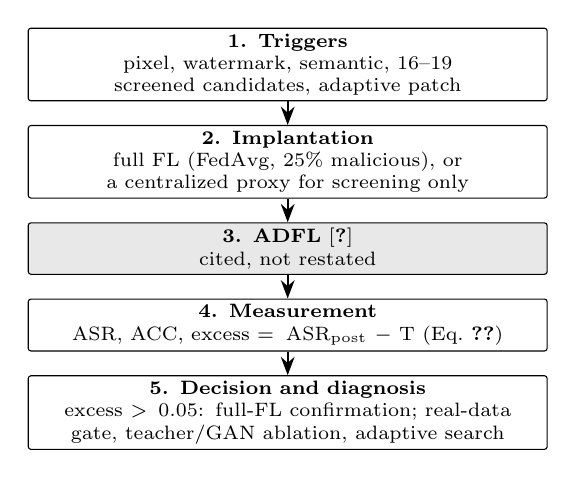
\begin{tikzpicture}[font=\scriptsize, >=Stealth, node distance=0.3cm,
  box/.style={draw, rounded corners=1pt, align=center, text width=6.45cm, inner sep=2pt, minimum height=0.6cm},
  citebox/.style={box, fill=gray!18},
  arr/.style={->, thick}]
\node[box] (trig) {\textbf{1. Triggers}\\pixel, watermark, semantic, 16--19 screened candidates, adaptive patch};
\node[box, below=of trig] (implant) {\textbf{2. Implantation}\\full FL (FedAvg, 25\% malicious), or a centralized proxy for screening only};
\node[citebox, below=of implant] (adfl) {\textbf{3. ADFL} \cite{zhu2023adfl}\\cited, not restated};
\node[box, below=of adfl] (metric) {\textbf{4. Measurement}\\ASR, ACC, excess $=\ASR_{\mathrm{post}}-\Texc$ (Eq.~\ref{eq:excess})};
\node[box, below=of metric] (diag) {\textbf{5. Decision and diagnosis}\\excess $>0.05$: full-FL confirmation; real-data gate, teacher/GAN ablation, adaptive search};
\draw[arr] (trig)--(implant); \draw[arr] (implant)--(adfl);
\draw[arr] (adfl)--(metric); \draw[arr] (metric)--(diag);
\end{tikzpicture}
\caption{Evaluation pipeline of this paper. Stage 3 is Zhu et al.'s defense, used as given; the screen, metric and diagnostics around it are the protocol I designed.}
\label{fig:pipe}
\end{figure}

\textbf{Models.} Grayscale: three $3{\times}3$ convolutions (16, 32, 128 channels), LeakyReLU, two max-pools and a 256-unit FC layer, without batch normalization \cite{ioffe2015bn} so FedAvg does not average running statistics; CIFAR-10: ResNet18 \cite{he2016resnet}. The generator is DCGAN-style \cite{radford2016dcgan}, and the discriminator's trunk copies the backdoored feature extractor with a fresh real/fake head.

\textbf{GAN and teacher.} BCE GAN training with Adam \cite{kingma2015adam} ($\beta_1=0.5$) and one-sided label smoothing \cite{salimans2016improved}; for CIFAR-10 also two-timescale rates \cite{heusel2017ttur}, two generator steps per discriminator step and decaying instance noise \cite{sonderby2017amortised}. The teacher uses Adam (40 epochs) for grayscale and SGD with Nesterov momentum, cosine annealing \cite{loshchilov2017sgdr} and augmentation (70 epochs) for CIFAR-10. The $N_{\mathrm{distill}}=10{,}000$ generated samples are labeled by the teacher's argmax.

\textbf{Distillation.} The student, a fresh copy of the backdoored model, minimizes
\begin{equation}
\mathcal{L}=\mathrm{CE}\big(s(x),\hat y\big)+\alpha\,T^{2}\,\mathrm{KL}\!\left(\sigma(f(x)/T)\,\Vert\,\sigma(s(x)/T)\right),
\label{eq:loss}
\end{equation}
with $T=3$, $\alpha=0.5$ \cite{hinton2015kd}. I train the GAN and distill once on the final global model, the ``distill only in the last round'' option noted in \cite{zhu2023adfl}.

\subsection{Attacks and Metrics}
The pixel attack is a BadNets-style \cite{gu2017badnets} $5{\times}5$ white block (target class 1 for grayscale, 0 for CIFAR-10). The watermark attack blends a ``1'' glyph, $(1-f)x+fw$ at $f=0.3$. The CIFAR-10 semantic attack follows \cite{bagdasaryan2020backdoor}: green-dominant automobiles are relabeled to class 0 without pixel changes (the test attribute subset has only 58 images).

$\ACC$ is clean test accuracy; $\ASR$ is the fraction of triggered test images, whose true label is not the target, assigned to the target. Let $\Texc$ be the clean teacher's own target rate on the same inputs. I define
\begin{equation}
\mathrm{excess}=\ASR_{\mathrm{post}}-\Texc,
\label{eq:excess}
\end{equation}
and call a backdoor \emph{surviving} if excess $>0.05$. The metric is trigger-agnostic: a trigger that already drives clean images to the target (large $\Texc$) cannot be mistaken for persistence. $\Texc$ uses the full test set in the main table and the first 2000 images in the screens.

\subsection{Evasion Screen and Real-Data Gate}
Because the defense is trigger-dependent, no single hand-picked attack characterizes it. Alg.~\ref{alg:screen} gives the screen I use instead: 16--19 candidates per dataset (random and white patches, stripes, dots, corner marks, noise) go through a centralized proxy, survivors are distilled with the main distillation set and ranked by excess, and only the top $k$ consume a full FL run. The proxy is one centralized model rather than an FL run, which is what makes the sweep affordable, but it overstates survival (excess $0.944$ versus $0.390$ under full FL), so it ranks candidates and is never reported as evidence. The real-data gate is a separate diagnostic: replacing the GAN samples by 10{,}000 \emph{real} training images relabeled by the same teacher separates a method failure from a data failure on CIFAR-10; it is not deployable, as the server would not hold those images.

\begin{algorithm}[t]
\caption{Trigger screen and full-FL confirmation (my protocol)}
\label{alg:screen}
\begin{algorithmic}[1]
\Require candidates $\mathcal{T}$ (16--19 per dataset), distillation set $D_{\mathrm{syn}}$
\For{$\tau\in\mathcal{T}$}
  \State Backdoor a centralized proxy with $\tau$; skip if its ASR is $<0.80$ or $\Texc(\tau)>0.20$
  \State Distill the proxy with $D_{\mathrm{syn}}$; record $\ASR_{\mathrm{post}}(\tau)$ and excess (Eq.~\ref{eq:excess})
\EndFor
\State Keep the top $k$ by excess ($k=3$; $k=2$ for CIFAR-10)
\State Implant each kept $\tau$ by full FL (25\% malicious), purify, and report ASR, ACC and excess over seeds 42--44
\end{algorithmic}
\end{algorithm}

\subsection{Adaptive Attack}
\label{sec:adaptivemethod}
The screen is blind to the defense, so I also built an adaptive attacker on Fashion-MNIST Non-IID (fixed Dirichlet-0.5 partition, paper fidelity, seeds 42--44). It searches a $14{\times}14$ raw-pixel patch with a $(\mu/\mu_w,\lambda)$ evolution strategy (60 generations, $\lambda=16$, 4{,}000 reference images): each generation mutates the current best patches, scores them, and keeps the $\mu$ best. The premise is that ADFL scrubs only behavior covered by the generator's distillation set, so a patch far from it should survive; the objective is a \emph{coverage} score, the input-space pixel MSE between the patch region and the corresponding region of distillation-set or real samples, which the search maximizes. % TODO: confirm exact coverage formula and what "min/mean" aggregates over
In the \emph{oracle} model the attacker optimizes against the server's actual distillation set and teacher; in the \emph{surrogate} model it trains its own teacher$'$ and GAN$'$ and transfers the patch. Each winner is implanted by full FL, purified by the complete pipeline and compared with a matched static baseline (the random $14{\times}14$ trigger at location $(7,7)$). Two earlier objectives were abandoned: one maximizing a proxy-KD excess overfit the proxy (post-ADFL ASR $0.096$), and a fast-tier diagnostic showing an apparent advantage (static $0.036$ vs.\ adaptive $0.174$) did not carry over to paper fidelity, so only paper-tier numbers are reported.

%=====================================================================
\section{Results}
\subsection{Experimental Setup}
All runs are in PyTorch \cite{paszke2019pytorch} on an RTX 3090 Ti with per-stage validated checkpoints: run of record 2026-10-17, follow-up 2026-10-30, adaptive 2026-11-01. Table~\ref{tab:hp} lists the paper-fidelity configuration; FL uses SGD with momentum 0.9, batch size 256, and FedAvg weighting by shard size. Rows are mean $\pm$ sample std.\ ($n-1$) over seeds 42--44, single-seed rows marked; with $n=3$ I report no hypothesis tests and make no significance claims. In the run of record the partition and teacher are fixed across seeds. Code and results will be released at [repository URL].

\begin{table}[t]
\centering
\caption{Paper-tier configuration.}
\label{tab:hp}
\footnotesize
\setlength{\tabcolsep}{2pt}
\begin{tabular}{lcc}
\toprule
Parameter & MNIST / Fashion & CIFAR-10 \\
\midrule
Clients / malicious / per round & 100 / 25 / 10 & 50 / 12 / 10 \\
FL rounds / local epochs & 200 / 20 & 100 / 10 \\
$\gamma$, poison rate, local lr & 1.5, 0.5, 0.01 & 1.5, 0.5, 0.01 \\
Teacher data / GAN data & 3\% / 10\% & 10\% / 20\% \\
GAN epochs, $N_{\mathrm{distill}}$ & 30, 10{,}000 & 120, 10{,}000 \\
KD epochs / lr / $T$ / $\alpha$ & 20 / $10^{-3}$ / 3 / 0.5 & 8 / $5{\times}10^{-4}$ / 3 / 0.5 \\
\bottomrule
\end{tabular}
\end{table}

\subsection{Reproduction and Non-IID Degradation}
For the reproduction and extension results, the MNIST pixel control passes (ASR $1.000\to0.002\pm0.002$, accuracy $0.990\to0.945$). Under IID data the Fashion-MNIST pixel trigger is only partly removed ($0.145\pm0.170$; per seed 0.335, 0.006, 0.095) while the watermark is removed ($0.001\pm0.001$); under Dirichlet partitioning the watermark survives ($0.074\pm0.027$, excess $+0.060$), the pixel trigger survives at $0.152\pm0.136$, and accuracy falls from 0.89 to 0.65--0.66.

Table~\ref{tab:main} reports the triggers designed in this work, all full-FL-confirmed (Alg.~\ref{alg:screen}). Among them, every IID grayscale candidate collapses over three seeds (largest mean 0.077, horizontal stripes), whereas under Non-IID a random $14{\times}14$ patch survives at $0.434\pm0.175$ (excess $+0.390$) and three corner marks retain $0.123\pm0.034$. The proxy overstates survival (excess 0.944 versus 0.390 under full FL), so full-FL confirmation is necessary. On CIFAR-10 a random $20{\times}20$ center patch reaches ASR 0.505, but at 0.182 accuracy, so it is uninformative.

\begin{table*}[t]
\centering
\caption{Designed triggers, full-FL-confirmed (Alg.~\ref{alg:screen}). Fashion-MNIST rows are mean $\pm$ sample std.\ ($n-1$) over seeds 42--44; MNIST and CIFAR-10 rows are single-seed. Pre-defense ASR is $\approx1.000$ for every trigger; $\Texc$ is the clean teacher's target rate on the first 2000 test images; excess $=$ ASR post $-$ $\Texc$.}
\label{tab:main}
\small
\setlength{\tabcolsep}{5pt}
\begin{tabular}{lllcccc}
\toprule
Partition & Dataset & Attack / trigger & ASR post & ACC pre$\to$post & $\Texc$ & Excess \\
\midrule
\multicolumn{7}{@{}l}{\emph{Fashion-MNIST, Non-IID (Dirichlet $\alpha=0.5$)}}\\
Non-IID & Fashion & random $14{\times}14$ pixel & $\mathbf{0.434\pm0.175}$ & $0.895\to0.671$ & 0.043 & $\mathbf{+0.390}$ \\
Non-IID & Fashion & three corners & $0.123\pm0.034$ & $0.896\to0.681$ & 0.002 & $+0.121$ \\
Non-IID & Fashion & random $20{\times}20$ pixel & $0.055\pm0.094$ & $0.898\to0.680$ & 0.000 & $+0.055$ \\
\midrule
\multicolumn{7}{@{}l}{\emph{Fashion-MNIST, IID}}\\
IID & Fashion & horizontal stripes & $0.077\pm0.128$ & $0.913\to0.743$ & 0.000 & $+0.077$ \\
IID & Fashion & random $14{\times}14$ center & $0.024\pm0.040$ & $0.911\to0.735$ & 0.000 & $+0.024$ \\
\midrule
\multicolumn{7}{@{}l}{\emph{MNIST, IID (control, single seed)}}\\
IID & MNIST & horizontal stripes & 0.078 & $0.990\to0.947$ & 0.000 & $+0.078$ \\
IID & MNIST & vertical stripes & 0.030 & $0.991\to0.944$ & 0.019 & $+0.011$ \\
IID & MNIST & three corners & 0.000 & $0.990\to0.946$ & 0.003 & $-0.003$ \\
\midrule
\multicolumn{7}{@{}l}{\emph{CIFAR-10, IID (single seed, ACC collapsed)}}\\
IID & CIFAR-10 & random $20{\times}20$ center & 0.505 & $0.636\to0.182$ & 0.000 & $+0.505$ \\
IID & CIFAR-10 & vertical stripes & 0.020 & $0.642\to0.177$ & 0.000 & $+0.020$ \\
\bottomrule
\end{tabular}
\end{table*}


\subsection{CIFAR-10: Diagnosing the Failure}
On CIFAR-10 ADFL lowers ASR but destroys the model: the pixel backdoor's accuracy falls from 0.64 to 0.15 and stays at 0.134--0.147 for every learning rate in Table~\ref{tab:cifar} (seed 42). Fig.~\ref{fig:gan} shows why: the CIFAR-10 generator produces low-diversity samples with a few recurring modes. Real teacher-relabeled data at the same rates remove the backdoor and keep 0.716--0.725 accuracy (Table~\ref{tab:cifar}), and even a teacher at 0.861 (20\% clean data) leaves GAN-based distillation at 0.190. The failure is thus attributable to the quality of the synthetic distillation data, not to the trigger or to distillation as such.

\begin{table}[t]
\centering
\caption{CIFAR-10 pixel attack (seed 42; backdoored ACC 0.642, ASR 0.978; teacher ACC 0.737). GAN rows at $4{\times}10^{-3}$ and $8{\times}10^{-3}$: ACC 0.143/0.147, ASR 0.027/0.025.}
\label{tab:cifar}
\footnotesize
\setlength{\tabcolsep}{4pt}
\begin{tabular}{lcccc}
\toprule
 & \multicolumn{2}{c}{GAN data} & \multicolumn{2}{c}{Real relabeled data} \\
\cmidrule(lr){2-3}\cmidrule(lr){4-5}
KD lr & ACC & ASR & ACC & ASR \\
\midrule
$5{\times}10^{-4}$ & 0.141 & 0.026 & 0.716 & 0.055 \\
$1{\times}10^{-3}$ & 0.134 & 0.010 & 0.725 & 0.028 \\
$2{\times}10^{-3}$ & 0.137 & 0.018 & 0.716 & 0.030 \\
\bottomrule
\end{tabular}
\end{table}

\begin{figure}[t]
\centering
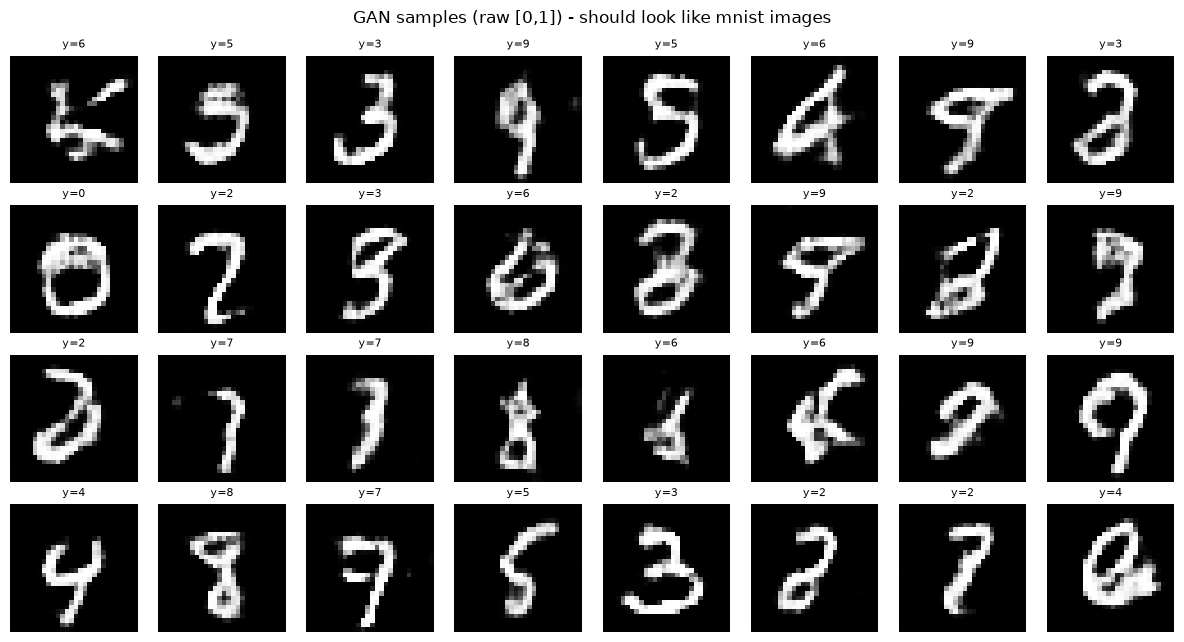
\includegraphics[width=0.31\columnwidth]{figures/gan_samples_mnist.png}\hfill
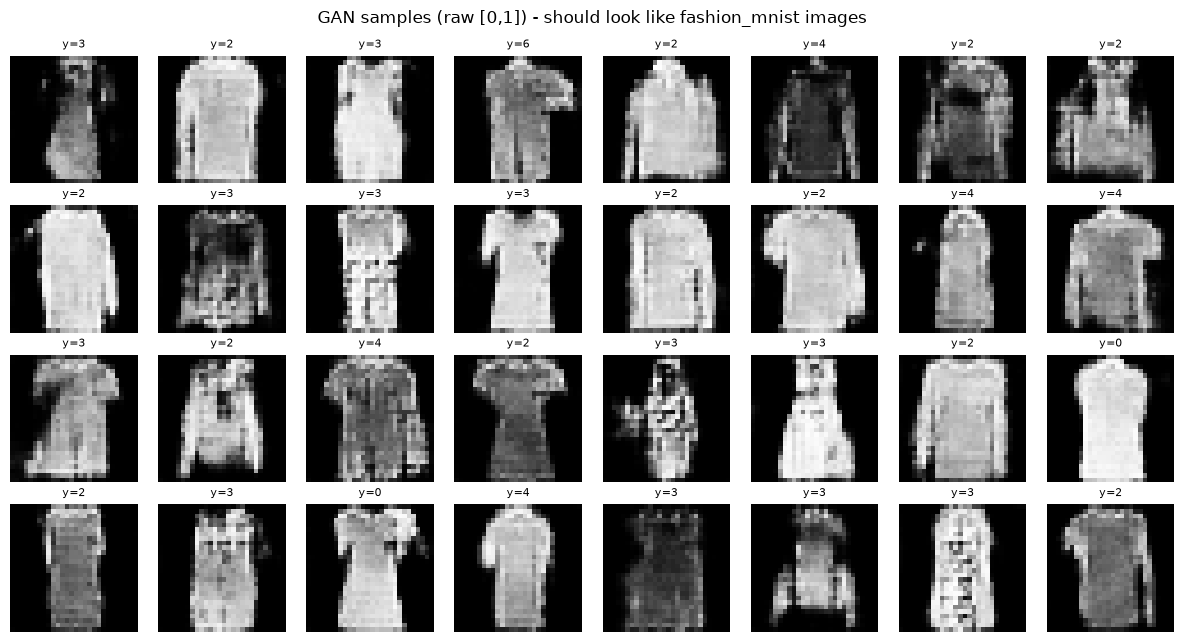
\includegraphics[width=0.31\columnwidth]{figures/gan_samples_fashion.png}\hfill
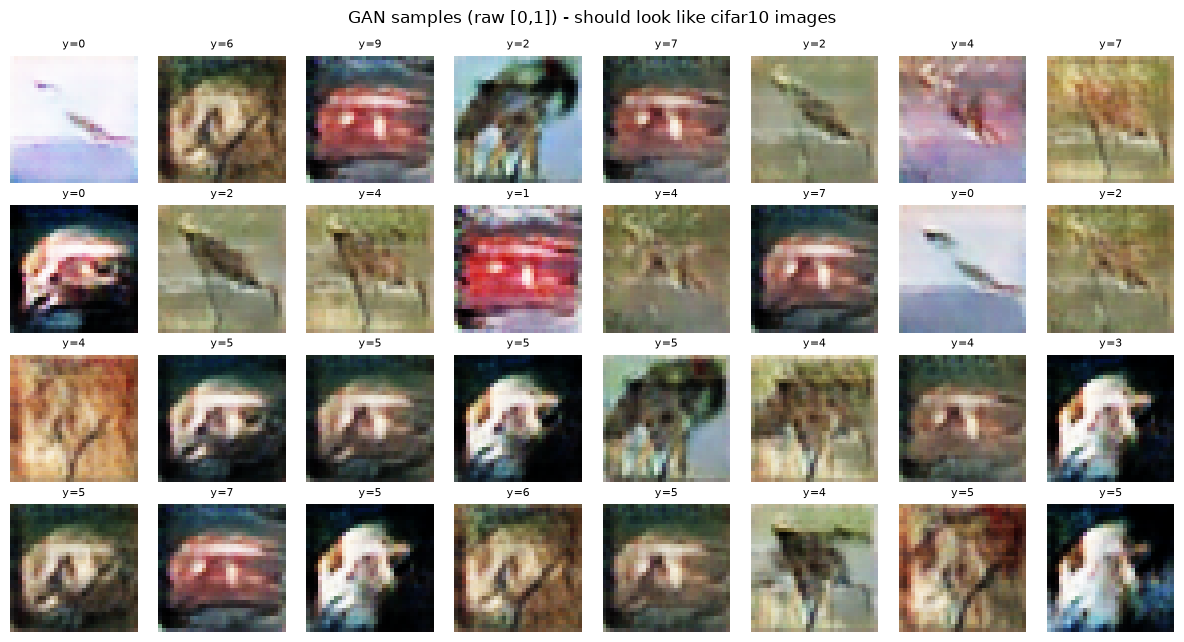
\includegraphics[width=0.31\columnwidth]{figures/gan_samples_cifar.png}
\caption{Generator samples with teacher labels (MNIST, Fashion-MNIST, CIFAR-10). The CIFAR-10 samples are low in diversity; this is the failure the real-data gate isolates.}
\label{fig:gan}
\end{figure}

\subsection{Follow-up: Multi-Seed Study and Ablations}
The follow-up keeps the configuration of Table~\ref{tab:hp} but redraws the client partition and teacher per seed, so its numbers differ from the fixed-partition run by design. \textbf{CIFAR-10, three seeds:} accuracy falls from $\approx0.65$ to $0.22$--$0.23$ for every seed (pixel $0.645\to0.225\pm0.101$; semantic $0.659\to0.229\pm0.090$), with a noisy post-ASR (pixel $0.480\pm0.343$), so the collapse is not a single-seed artifact. \textbf{Redrawn Non-IID:} the MNIST pixel backdoor is removed even under Non-IID data (ASR $0.9998\to0.009\pm0.003$, accuracy $0.988\to0.948$), so the grayscale failure is not a generic consequence of partitioning. The Fashion watermark, which survived at $0.074\pm0.027$ under one fixed partition, is removed on average ($0.010\pm0.010$), whereas the random $14{\times}14$ patch survives at $0.188\pm0.326$, a mean dominated by one retaining seed; the partition and teacher draw are thus a first-order variance source.

\textbf{Teacher versus GAN.} Table~\ref{tab:ablation} fixes the Non-IID backdoored Fashion-MNIST model and varies whether the teacher's and the GAN's clean samples are IID or Non-IID. A Non-IID \emph{teacher} drops post-defense accuracy to $\approx0.50$ and roughly doubles residual ASR, whereas changing the GAN's partition barely matters.

\begin{table}[t]
\centering
\caption{Teacher vs.\ GAN-data partition ablation, Non-IID Fashion-MNIST (pixel attack, 3 seeds). ASR: mean $\pm$ std; ACC: mean.}
\label{tab:ablation}
\small
\setlength{\tabcolsep}{6pt}
\begin{tabular}{llcc}
\toprule
Teacher & GAN & ASR post & ACC post \\
\midrule
IID & IID & $0.118\pm0.066$ & 0.638 \\
IID & Non-IID & $0.118\pm0.062$ & 0.652 \\
Non-IID & IID & $0.200\pm0.089$ & 0.498 \\
Non-IID & Non-IID & $0.148\pm0.035$ & 0.497 \\
\bottomrule
\end{tabular}
\end{table}

\begin{figure}[t]
\centering
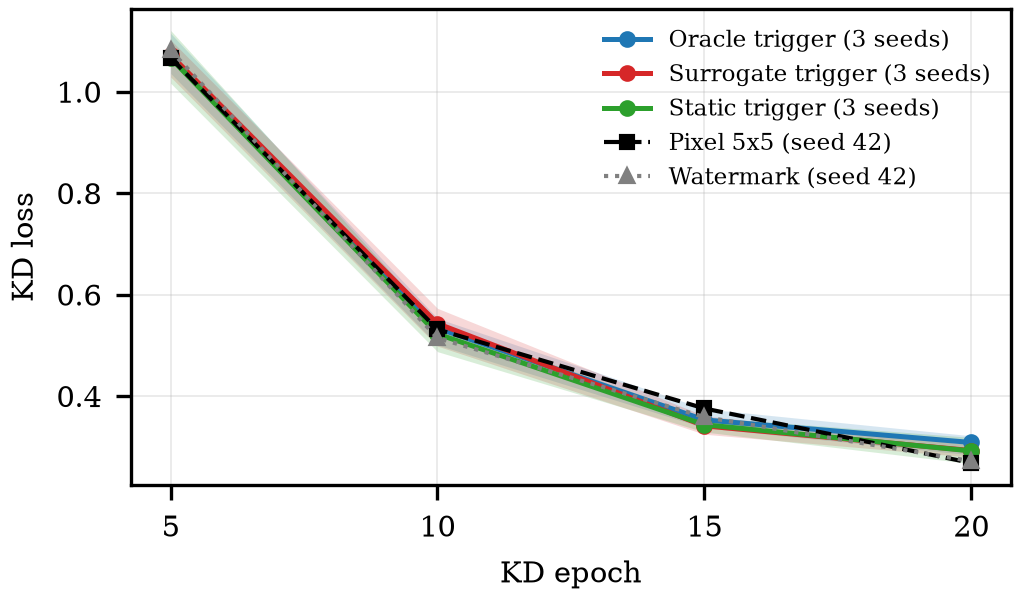
\includegraphics[width=0.78\columnwidth]{figures/kd_loss.png}
\caption{KD loss versus distillation epoch, Fashion-MNIST Non-IID. Means over seeds 42--44 for the adaptive conditions (bands: min--max); seed 42 for the pixel and watermark triggers.}
\label{fig:kd}
\end{figure}

\textbf{Distillation loss.} Fig.~\ref{fig:kd} shows the KD objective $\mathcal{L}_{\mathrm{hard}}+\alpha\mathcal{L}_{\mathrm{soft}}$ (epoch-averaged): it falls from about $1.0$--$1.1$ at epoch 5 to $0.27$--$0.32$ at epoch 20 in every run, and its trajectory is indistinguishable across the pixel, watermark, static, oracle and surrogate triggers. The student thus fits the GAN-generated set equally well whether or not the backdoor survives (post-ASR $0.11$--$0.53$), so the loss carries no information about residual backdoor strength.

\subsection{Adaptive Attack: A Negative Result}
\label{sec:adaptive}
Table~\ref{tab:adaptive} gives the paper-tier result. Neither adaptive trigger beats the matched static baseline: the oracle trigger retains $0.416\pm0.292$ ASR and the surrogate $0.373\pm0.353$, against $0.526\pm0.268$ for the static trigger. With three seeds and standard deviations of $0.27$--$0.35$ these differences are within noise, so the supportable claim is \emph{no advantage} over a blind static trigger; the ordering of oracle and surrogate is uninformative. The search raised oracle coverage from $0.169$ to $0.551$ (min/mean $0.423/0.513$ versus $0.090/0.170$), yet survival did not increase, so input-space distance from the distillation set is not a useful proxy for what distillation fails to remove, at least for this patch family. The static baseline here differs from the $0.434\pm0.175$ of Table~\ref{tab:main} for the same trigger, implying a run-to-run spread of roughly $0.09$ in the mean at this seed count. % TODO: confirm whether the two runs share backdoored FL checkpoints (acc_pre 0.8973 here vs 0.895 in Table main suggests they do not)
ADFL costs similar clean accuracy regardless of trigger ($\approx0.90\to0.66$--$0.70$).

\begin{table}[t]
\centering
\caption{Adaptive attack, Fashion-MNIST Non-IID ($\alpha=0.5$), seeds 42--44, paper fidelity (mean $\pm$ sample std). ASR pre is 1.000 and ACC pre $\approx0.897$ in all conditions; coverage is min/mean as logged.}
\label{tab:adaptive}
\footnotesize
\setlength{\tabcolsep}{2pt}
\begin{tabular}{lcccc}
\toprule
Trigger & ASR post & ACC post & Excess & Coverage \\
\midrule
Static (matched) & $0.526\pm0.268$ & $0.702\pm0.024$ & $+0.483$ & 0.090/0.170 \\
Adaptive, oracle & $0.416\pm0.292$ & $0.660\pm0.062$ & $+0.357$ & 0.423/0.513 \\
Adaptive, surrogate & $0.373\pm0.353$ & $0.683\pm0.033$ & $+0.373$ & 0.338/0.466 \\
\bottomrule
\end{tabular}
% TODO: per-seed post-ADFL ASR to be recovered from the saved purified checkpoints.
\end{table}

%=====================================================================
\section{Discussion}

\textbf{The accuracy tax.} Post-defense accuracy falls short of the original ``above 90\%'' everywhere: $-0.04$ on MNIST, $-0.16$ on Fashion IID, $-0.24$ on Fashion Non-IID, and a collapse on CIFAR-10. In every grayscale case it sits at or below the teacher's (0.958, 0.784, 0.771), consistent with the student being pulled toward a weak teacher trained on 3\% of the data.

\textbf{Why Non-IID hurts.} Table~\ref{tab:ablation} localizes the cause in the server teacher: a small clean sample from a skewed partition yields a weak teacher that distillation cannot exceed. The MNIST Non-IID control is still cleaned, so partitioning alone does not break the defense; failure appears where the teacher's sample is heterogeneous \emph{and} the task is hard enough. Survival under one fixed partition can mislead, as the watermark case shows.

\textbf{CIFAR-10.} The failure is a property of the synthetic data in my setup (a reduced-compute generator on a small clean sample), not of distillation, and need not hold for stronger generators.

\textbf{Adaptive attacker.} The bounded study found no trigger better than a blind random one, so it does not show that ADFL is adaptively robust: it tests one objective, one patch family and one dataset. It does show that the distance-based intuition is unsupported and that seed spread exceeds any trigger difference I could produce.

\textbf{Limitations.} (i)~Three seeds make standard deviations large: the adaptive study cannot resolve mean-ASR differences below roughly $0.3$, and fixed-partition standard deviations are lower bounds. (ii)~The CIFAR-10 gate and sweeps are single-seed on a reduced tier (50 clients, 100 rounds), the collapsed accuracy makes post-ASR uninformative there, and the semantic backdoor is weak (58 test images). (iii)~The server uses extra clean data (13\% grayscale, 30\% CIFAR-10), purification is single-shot, and I did not run baseline defenses, DBA or WaNet, so Zhu et al.'s comparisons are not reproduced. No reference implementation exists, so my pipeline is a reconstruction from the paper's description and undocumented design choices are mine. (iv)~The proxy screen is not a faithful predictor of full-FL survival, and the static baseline differs by about $0.09$ between runs, so single-run survival numbers carry at least that uncertainty. (v)~The Fashion-MNIST clean-budget sweeps in the result files came from an earlier run and are not reported.

%=====================================================================
\section{Conclusions}
On an MNIST pixel control ADFL behaves as reported, but in my hands its protection weakens under Non-IID data, a trigger found by my screen survives at $0.434$ ASR ($0.526\pm0.268$ on a matched re-run, with very large seed-to-seed spread), and on CIFAR-10 the GAN-generated distillation data cannot support a usable purified model although real relabeled data can. A follow-up confirms the CIFAR-10 collapse across three seeds, traces the Non-IID degradation to the teacher rather than the GAN data, and shows that an MNIST Non-IID control is still cleaned, so dataset complexity, not partitioning per se, governs where the defense breaks. A bounded adaptive attack did not beat a blind random trigger, so whether ADFL can be defeated adaptively remains open. \textbf{Future work:} stronger generators for CIFAR-10, adaptive attackers with feature-space objectives, and head-to-head evaluation against the baselines of the original paper.

\bibliographystyle{IEEEtran}
\bibliography{refs}

\end{document}